\documentclass[a4paper,10pt]{book}
\usepackage[centertags]{amsmath}
\usepackage{amscd}
\usepackage{amsthm}
\usepackage{amssymb}
\usepackage{enumerate}
\usepackage{multicol}
\usepackage[english,catalan,spanish]{babel}
\usepackage[all]{xy}
\usepackage{color}
\usepackage{tikz}
\usepackage{indentfirst}
\usepackage[utf8]{inputenc}
\usepackage[T1]{fontenc}
\linespread{1.1}
\setlength{\parskip}{10pt}
\usepackage[twoside,bindingoffset=1cm]{geometry}
\usepackage{lmodern}
\usepackage[x11names, dvipsnames, table]{xcolor}
\definecolor{ubblue}{HTML}{0059A2}
\usepackage[colorlinks=true, linkcolor=black, citecolor=ubblue, urlcolor=ubblue]{hyperref}
\usepackage{cleveref}
\usepackage[protrusion=true,expansion=true]{microtype}
\usepackage{cite}



%% Custom packages


%%%%%%%%%%%%%%%%%%%%%%%%%%%%%%%%%%%%%%%%%%%%%%%%%%%%%%%%%%%%%%%%%%%%%%%%%%%
%%%% local definitions for this paper
%%%%%%%%%%%%%%%%%%%%%%%%%%%%%%%%%%%%%%%%%%%%%%%%%%%%%%%%%%%%%%%%%%%%%%%%%%%


%%%%%%%%%%%%%%%%%%%%%% aix{\`o} pels headings %%%%%%%%%%%%%%%%%%%%%%%%
\usepackage{fancyhdr}
\pagestyle{fancy}
\renewcommand{\chaptermark}[1]{\markboth{#1}{}}
\renewcommand{\sectionmark}[1]{\markright{\thesection\ #1}}
\fancyhf{} \fancyhead[LE,RO]{\bfseries\thepage}
\fancyhead[LO]{\bfseries\rightmark} \fancyhead[RE]{\bfseries\leftmark}

\def\paginaenblanc{\newpage%
\thispagestyle{empty}%
\vspace*{2cm}%
\newpage%
\thispagestyle{empty}%
}


%%%%%%%%%%%%%%%%%%%%%%%%%%%%%%%%%%%%%%%%%%%%%%%%%%%%%%%%%%%%%%%%%%%%%%%%%
% aux commands
%%%%%%%%%%%%%%%%%%%%%%%%%%%%%%%%%%%%%%%%%%%%%%%%%%%%%%%%%%%%%%%%%%%%%%%%%
%==========================================================================
% macros to support private authors' notes
%==========================================================================
\newif\ifprivate
\privatetrue
\def\xbar{\vskip0.09in\hrule\vskip0.06in}
\def\private#1{\ifprivate \xbar {\em #1} \xbar
\else \fi}
\def\huh{\ifprivate ??? \marginpar{\Huge ???}
\else \fi}
\def\???{\ifprivate {\bf {???}} \marginpar{\begin{center}{\Huge {\bf ?}}\end{center}}
\else \fi}
%\def\???{\ifprivate {\bf {???}} \marginpar{{\Huge {\bf ?}}}
%\else \fi}
\marginparsep1mm
\def\nota#1{\ifprivate  $\clubsuit$ \marginpar{\parbox[t]{2.4cm}{\begin{center}\tiny #1\end{center}}}
\else \fi}
\def\comment#1{\ifprivate \marginpar{\parbox[t]{2.4cm}{\begin{center}\tiny #1\end{center}}}
\else \fi}
%\def\nota#1{\ifprivate  $\clubsuit$ \marginpar{\parbox[t]{1.8cm}{\tiny #1}}
%\else \fi}
\def\privateeject{\ifprivate\eject\fi}
%\def\???{{\bf {???}} \marginpar{{\Huge {\bf ?}}} }
%%%%%%%%%%%%%%%%%%%%%%%%%%%%%%%%%%%%%%%%%%%%%%%%%%%%%%%%%%%%%%%%%%%%%%%%%%

%%%%%%%%%%%%%%%%%%%%%%%%%%%%%%%%%%%%%%%%%%%%%%%%%%%%%%%%%%%%%%%%%%%%%%%%
%%%%%%%%%%%%%%%%%%%%%%%%%%%%%%%%%%%%%%%%%%%%%%%%%%%%%%%%%%%%%%%%%%%%%%%%
\begin{document}

\pagestyle{empty}

\begin{titlepage}
	\begin{center}
		\begin{figure}[htb]
			\begin{center}
				
\includegraphics[width=6cm]{assets/ub_color.pdf}
			\end{center}
		\end{figure}
		
		\def\worktitle{Development of an AI-Based Tool for Molecular Subtype Classification of Invasive Ductal Breast Carcinoma Using Mammography}
		
		\textbf{\LARGE Treball final de grau} \\
		\vspace*{.5cm}
		\textbf{\LARGE GRAU D'ENGINYERIA INFORM\`{A}TICA } \\
		\vspace*{.5cm}
		\textbf{\LARGE Facultat de Matem\`atiques i Inform\`atica\\ Universitat de Barcelona} \\
		\vspace*{1.0cm}
		\rule{16cm}{0.1mm}\\
		\begin{Huge}
			\textbf{Evaluation of Transformer-Based Models for Molecular Subtype Classification of Invasive Ductal Breast Carcinoma Using Mammography} \\
		\end{Huge}
		\rule{16cm}{0.1mm}\\
		
		\vspace{1cm}
		
		\begin{flushright}
			
			
			\vspace*{2.5cm}
			
			\hfill
			
			\renewcommand{\arraystretch}{1.5}
			\begin{tabular}{ll}
				\textbf{\small Autor:}       & \textbf{\small David Bland\'on T\'orrez }                             \\
				\textbf{\small Director:}    & \textbf{\small Dr. Oliver D\'iaz Montesdeoca }                        \\
				\textbf{\small Realitzat a:} & \textbf{\small  Departament de Matem\`{a}tiques i  Inform\`{a}tica  } \\
				\textbf{\small Barcelona,}   & \textbf{\small \today }                                               
			\end{tabular}
			
		\end{flushright}
		
	\end{center}
	
\end{titlepage}

%%%%%%%%%%%%%%%%%%%%%%%%%%%%%%%%%%%%%%%%%%%%%%%%%%%%%%%%%%%%%%%%%%%%%%%%%
\newpage
\selectlanguage{spanish}
\noindent \textbf{\large Resumen}

// TODO

%%%%%%%%%%%%%%%%%%%%%%%%%%%%%%%%%%%%%%%%%%%%%%%%%%%%%%%%%%%%%%%%%%%%%%%%%

%%%%%%%%%%%%%%%%%%%%%%%%%%%%%%%%%%%%%%%%%%%%%%%%%%%%%%%%%%%%%%%%%%%%%%%%%
\newpage
\selectlanguage{english}
\noindent \textbf{\large Abstract}

// TODO

%%%%%%%%%%%%%%%%%%%%%%%%%%%%%%%%%%%%%%%%%%%%%%%%%%%%%%%%%%%%%%%%%%%%%%%%%

%%%%%%%%%%%%%%%%%%%%%%%%%%%%%%%%%%%%%%%%%%%%%%%%%%%%%%%%%%%%%%%%%%%%%%%%%
\newpage
\selectlanguage{catalan}
\noindent \textbf{\large Resum}

// TODO

%%%%%%%%%%%%%%%%%%%%%%%%%%%%%%%%%%%%%%%%%%%%%%%%%%%%%%%%%%%%%%%%%%%%%%%%%
\newpage
\selectlanguage{spanish}
\noindent \textbf{\large Agradecimientos}

// TODO
%%%%%%%%%%%%%%%%%%%%%%%%%%%%%%%%%%%%%%%%%%%%%%%%%%%%%%%%%%%%%%%%%%%%%%%%%
\selectlanguage{spanish}
\pagenumbering{roman} \setcounter{page}{0}
\let\cleardoublepage\clearpage
\tableofcontents
\newpage \thispagestyle{empty}
%%%%%%%%%%%%%%%%%%%%%%%%%%%%%%%%%%%%%%%%%%%%%%%%%%%%%%%%%%%%%%%%%%%%%%%%%

%%%%
%\listoffigures
%%%

\pagestyle{fancy}
\markboth{Introducción}{Introducción}
\newpage \thispagestyle{empty}
%%%%%%%%%%%%%%%%%%%%%%%%%%%%%%%%%%%%%%%%%%%%%%%%%%%%%%%%%%%%%%%%%%%%%%%%%
\mainmatter
\chapter{Introducción}
\section{Contexto}

El cáncer de mama se ha consolidado como una de las principales causas de mortalidad entre las mujeres y representa el tipo de cáncer con mayor incidencia en esta población. Se estima que, en promedio, una de cada veinte mujeres a nivel mundial será diagnosticada con esta enfermedad a lo largo de su vida \cite{kim_global_2025}. Proyecciones recientes sugieren que, de mantenerse la tendencia actual, para el año 2050, se registrarán aproximadamente 3.2 millones de nuevos casos y 1.1 millones de muertes asociadas a esta patología, con un impacto especialmente significativo en los países con bajo índice de desarrollo humano (HDI) \cite{kim_global_2025}.

Ante este panorama, las técnicas y herramientas de diagnóstico temprano desempeñan un papel fundamental para mejorar el pronóstico y supervivencia de las pacientes \cite{wang_early_2017}. Sin embargo, el cáncer de mama es una enfermedad heterogénea\footnote{Diversidad celular presente dentro de un tumor (heterogeneidad intratumoral) o entre diferentes tumores en un mismo individuo (heterogeneidad intertumoral).} que puede clasificarse en diversos subtipos según características clínicas y, especialmente, moleculares. Las guías internacionales del Consenso de St. Gallen de 2013 \cite{goldhirsch_personalizing_2013} reconocen cuatro subtipos principales basados en receptores hormonales (estrógeno, progesterona) y el marcador de proliferación Ki67: Luminal A, Luminal B, HER2 positivo (HER2-enriched) y Triple Negativo (véase figura \ref{fig:subtypes}). Esta clasificación tiene implicaciones clínicas directas, ya que el pronóstico, la respuesta a la terapia y las opciones de tratamiento dependen en gran medida del subtipo molecular al que pertenezca el tumor.

Actualmente, la caracterización molecular del tumor se realiza principalmente mediante biopsia, un procedimiento invasivo y costoso que, en ocasiones, debe repetirse, lo que puede retrasar el inicio del tratamiento e incrementar la carga clínica, física y emocional de las pacientes. Por ello, existe una necesidad creciente de desarrollar métodos no invasivos, accesibles y eficientes que permitan realizar esta tarea de manera fiable. En este sentido, la mamografía se posiciona como herramienta clave, ya que es una técnica no invasiva, de bajo coste y ampliamente utilizada en el diagnóstico temprano del cáncer de mama.


\begin{figure}
	\centering
	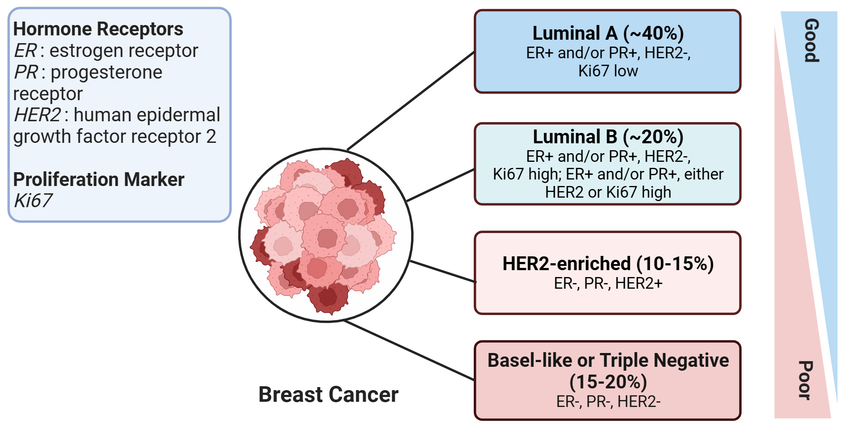
\includegraphics[width=0.8\linewidth]{reports/assets/subtypes.png}
	\caption{Los 4 subtipos moleculares del cáncer de mama y su porcentaje de relevancia \cite{harnessing_2024}}
	\label{fig:subtypes}
\end{figure}


En los últimos años, los avances en inteligencia artificial (IA), junto con la creciente disponibilidad de datos y una capacidad de cómputo cada vez más eficiente, han impulsado el desarrollo de modelos de aprendizaje profundo (DL) para tareas como la clasificación, detección y predicción del cáncer de mama, así como de otras enfermedades. Diversos estudios han demostrado que estos sistemas pueden igualar e incluso superar el desempeño de expertos humanos o sistemas CAD\footnote{Computer-Aided Diagnosis} en este tipo de tareas \cite{mckinney_international_2020,pattanaik_breast_2022,meenalochini_deep_2024,hussain_performance_2025}, lo que evidencia el impacto significativo de esta tecnología y su potencial beneficio para la práctica clínica y el bienestar de los pacientes.

Recientemente, se ha explorado la clasificación de subtipos moleculares a partir de imágenes mamográficas. Mota et al. (2024) \cite{mota_breast_2024} abordaron esta tarea, logrando un AUC del 60.62\% en clasificación multiclase con una arquitectura ResNet101. Por su parte, Rabah et al. (2025) \cite{ben_rabah_multimodal_2025} alcanzaron un AUC del 63.79\% aplicando un modelo Xception, y propusieron además un enfoque multimodal que integraba metadatos clínicos, elevando el rendimiento hasta un 88.87\% de AUC. Aunque los resultados obtenidos en escenarios unimodales son aún modestos y se encuentran por debajo del umbral de utilidad clínica establecido (\textasciitilde80\% AUC), estos estudios demuestran el potencial de la imagen como fuente diagnóstica y refuerzan la necesidad de continuar investigando en esta línea para mejorar la precisión y la utilidad clínica de estos modelos.

Este estudio propone un enfoque unimodal basado exclusivamente en mamografías del dataset público CMMD (The Chinese Mammography Database) \cite{cai_online_2023}, con el objetivo de comparar el rendimiento de arquitecturas Transformer de última generación como Vision Transformer (ViT), Shifted-Windows Transformer (SwinT) y Multi-Axis Vision Transformer (MaxViT), frente a un enfoque tradicional basado en redes convolucionales profundas (CNN). Aunque los modelos multimodales suelen lograr mejores resultados al integrar datos clínicos complementarios, centrarse únicamente en imágenes mamográficas presenta un alto valor práctico, especialmente en contextos con recursos limitados o donde la estandarización de los datos clínicos no está garantizada. Estudios recientes han evidenciado que los Transformers superan en precisión y robustez a las CNN en tareas de clasificación médica gracias a sus mecanismos de autoatención, que permiten capturar relaciones espaciales globales dentro de la imagen \cite{mauricio_comparing_2023}. Basándose en estas ventajas de diseño, este estudio plantea la hipótesis de que las arquitecturas Transformer podrían alcanzar un desempeño superior en la clasificación de subtipos moleculares, incluso bajo un enfoque unimodal.

En definitiva, este trabajo busca contribuir al desarrollo de herramientas diagnósticas no invasivas mediante la evaluación sistemática de modelos Transformer, con el fin de avanzar hacia una caracterización molecular automatizada, accesible y eficiente del cáncer de mama, especialmente en contextos donde la biopsia no es una opción inmediata, contribuyendo así a mejorar el acceso equitativo al diagnóstico y a reducir los tiempos de intervención terapéutica.

\section{Planificación}

\subsection{Definición de objetivos}

El \textbf{objetivo principal} de este estudio es explorar y evaluar el rendimiento de distintas arquitecturas de modelos del estado del arte basados en Transformers para la clasificación de subtipos moleculares del cáncer de mama a partir de mamografías, con el fin de contribuir al desarrollo de herramientas no invasivas que faciliten su caracterización. La premisa es que estos modelos se desempeñan mejor en tareas de clasificación y que sus mecanismos de atención podrían ayudar a capturar características relevantes que sirvan de apoyo para la caracterización tumoral.

Para alcanzar este objetivo, se plantean los siguientes \textbf{objetivos secundarios}:

\begin{enumerate}
	\item Revisar el estado del arte en la clasificación de subtipos moleculares mediante inteligencia artificial, identificando enfoques y resultados recientes.
	\item Implementar un pipeline de entrenamiento y evaluación, basado en validación cruzada, que permita estimar de forma robusta el rendimiento de modelos Transformer como ViT, SwinT y MaxViT.
	\item Analizar el impacto del desbalance de clases en el rendimiento de los modelos y aplicar técnicas de mitigación como el uso de funciones de pérdida ponderadas (\textit{weighted loss}), muestreo equilibrado (\textit{WeightedRandomSampler}) o aumentación de datos.
	\item Comparar los resultados obtenidos con un modelo convolucional de referencia (ResNet101), así como con estudios previos relevantes.
	\item Realizar un análisis estadístico que permita validar la significancia y la robustez de los resultados obtenidos.
	\item Aplicar técnicas de interpretabilidad como Grad-CAM o Attention Rollout sobre los modelos mejor desempeñados, para identificar regiones mamográficas asociadas a cada subtipo molecular.
	\item Interpretar y sintetizar los resultados obtenidos, proponiendo futuras mejoras y líneas de investigación alternativas.
\end{enumerate}


\subsection{Tareas a desarrollar}

\textbf{Estado del arte}

\begin{enumerate}
	\item Revisar la literatura científica actual sobre el cáncer de mama para contextualizar su relevancia clínica y epidemiológica.
	\item Analizar la importancia de la caracterización molecular del cáncer de mama, destacando sus ventajas, limitaciones y desafíos actuales.
	\item Examinar los avances recientes en el uso de inteligencia artificial y deep learning para la caracterización y diagnóstico del cáncer de mama, comparando enfoques y resultados reportados en la literatura.
\end{enumerate}

\textbf{Implementación}

\begin{enumerate}
	\item \textbf{Recolección de datos}: Obtención de las imágenes, conocer la estructura, organización y metadatos proporcionados por el dataset.
	\item \textbf{Análisis y preprocesamiento de datos}: Analizar la distribución de clases, coherencia de datos y realizar preprocesamiento de imágenes.
	\item \textbf{Codificación del proyecto}: Desarrollar el proyecto para llevar a cabo los experimentos, entrenamiento y evaluación de los diferentes modelos a evaluar.
	\item \textbf{Análisis de los resultados}: Comparar e interpretar los resultados obtenidos para plantear conclusiones y trabajos futuros.
\end{enumerate}

\textbf{Elaboración del reporte}

\begin{enumerate}
	\item \textbf{Escritura del reporte}: Escritura y documentación de los procedimientos llevados a cabo para realizar el proyecto, incluyendo metodología, materiales, resultados y conclusiones.
	\item \textbf{Correcciones}: Aplicar sugerencias ofrecidas por el tutor y refinar hasta alcanzar la calidad aceptada.
	\item \textbf{Entrega y presentación}: Entrega de la memoria y resumir los resultados más importantes para la presentación ante el comité.
\end{enumerate}

\subsection{Cronograma}

A continuación, se presenta el cronograma del proyecto, representado mediante un diagrama de Gantt que muestra las tareas previstas y su distribución temporal a lo largo del periodo de ejecución.

\begin{figure}[h!]
	\centering
	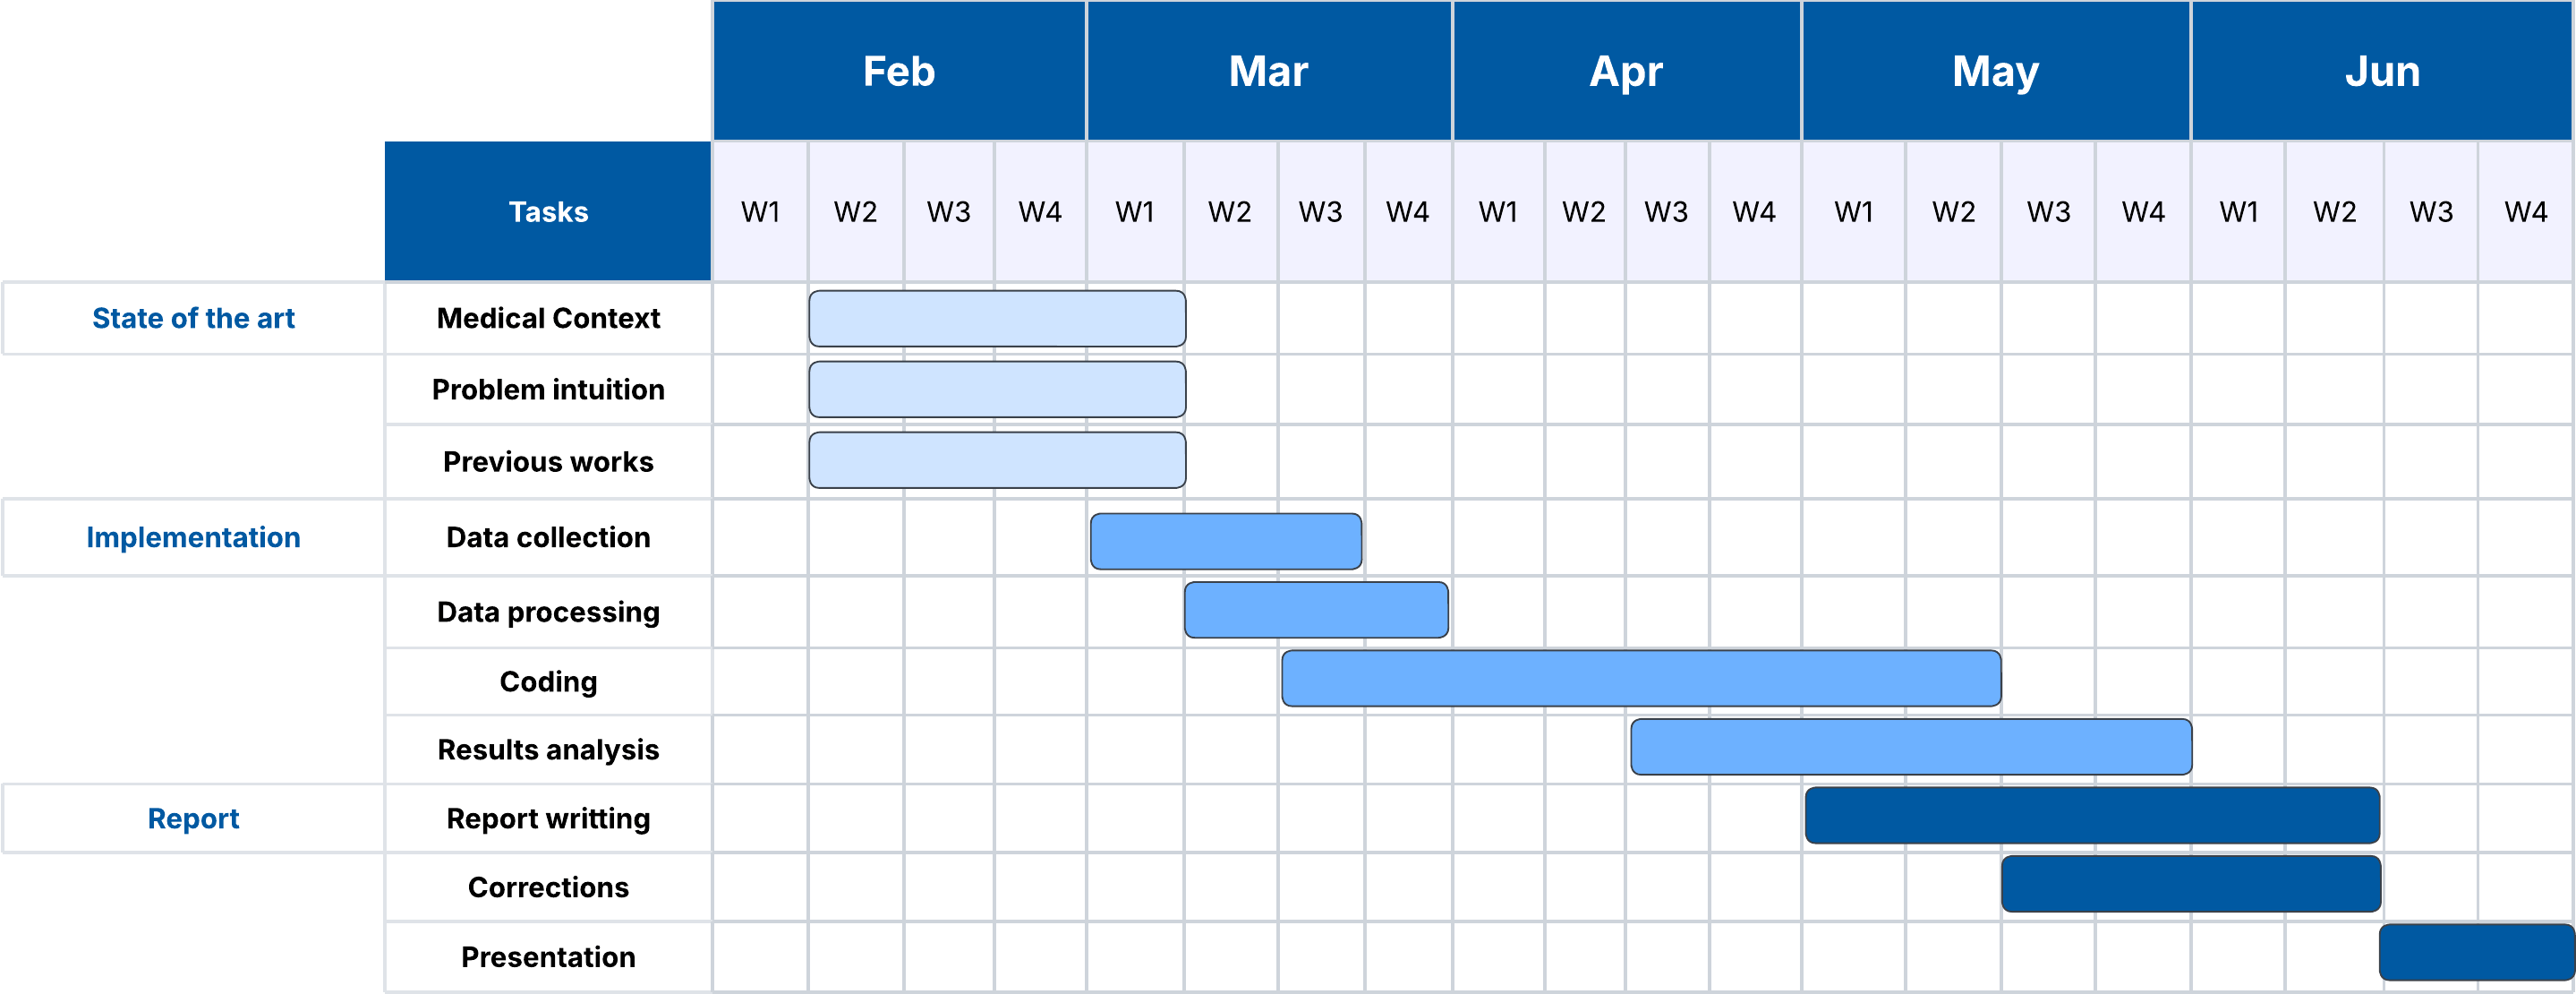
\includegraphics[width=1\linewidth]{reports//assets/RoadmapV3.png}
	\caption{Diagrama de Gantt}
	\label{fig:roadmap}
\end{figure}



%%%%%%%%%%%%%%%%%%%%%%%%%%%%%%%%%%%%%%%%%%%%%%%%%%%%%%%%%%%%%%%%%%%%%%%%%

\chapter{Antecedentes}

\section{Cáncer de mama: Contexto clínico y relevancia}
\section{Clasificación molecular del cáncer de mama}
\section{Mamografía y su rol en la caracterización tumoral}
\section{Inteligencia artificial en la imagen médica}
\section{Clasificación de subtipos moleculares mediante imagen}

\chapter{Revisión tecnológica}

Lorem ipsum dolor sit amet, consectetur adipiscing elit, sed do eiusmod tempor incididunt ut labore et dolore magna aliqua.


\section{Inteligencia artificial y aprendizaje profundo}
\subsection{De la IA clásica al Deep Learning}
Lorem ipsum dolor sit amet, consectetur adipiscing elit, sed do eiusmod tempor incididunt ut labore et dolore magna aliqua.
\subsection{Línea de tiempo}
Lorem ipsum dolor sit amet, consectetur adipiscing elit, sed do eiusmod tempor incididunt ut labore et dolore magna aliqua.

\section{Redes neuronales convolucionales}
Lorem ipsum dolor sit amet, consectetur adipiscing elit, sed do eiusmod tempor incididunt ut labore et dolore magna aliqua.
\subsection{Principios generales}
Lorem ipsum dolor sit amet, consectetur adipiscing elit, sed do eiusmod tempor incididunt ut labore et dolore magna aliqua.
\subsection{Arquitecturas y variantes históricas}
Lorem ipsum dolor sit amet, consectetur adipiscing elit, sed do eiusmod tempor incididunt ut labore et dolore magna aliqua.
\subsection{Limitaciones en mamografía}
Lorem ipsum dolor sit amet, consectetur adipiscing elit, sed do eiusmod tempor incididunt ut labore et dolore magna aliqua.

\section{Transformers para visión}
Lorem ipsum dolor sit amet, consectetur adipiscing elit, sed do eiusmod tempor incididunt ut labore et dolore magna aliqua.
\subsection{Breve historia}
Lorem ipsum dolor sit amet, consectetur adipiscing elit, sed do eiusmod tempor incididunt ut labore et dolore magna aliqua.
\subsection{Principios de la autoatención}
Lorem ipsum dolor sit amet, consectetur adipiscing elit, sed do eiusmod tempor incididunt ut labore et dolore magna aliqua.
\subsection{Vision Transformer (ViT)}
Lorem ipsum dolor sit amet, consectetur adipiscing elit, sed do eiusmod tempor incididunt ut labore et dolore magna aliqua.
\subsection{Shifted-Window Transformer (Swin)}
Lorem ipsum dolor sit amet, consectetur adipiscing elit, sed do eiusmod tempor incididunt ut labore et dolore magna aliqua.
\subsection{Multi-Axis Vision Transformer (MaxViT)}
Lorem ipsum dolor sit amet, consectetur adipiscing elit, sed do eiusmod tempor incididunt ut labore et dolore magna aliqua.
\section{Técnicas de entrenamiento y evaluación}
Lorem ipsum dolor sit amet, consectetur adipiscing elit, sed do eiusmod tempor incididunt ut labore et dolore magna aliqua.
\subsection{Transfer learning y fine-tuning}
Lorem ipsum dolor sit amet, consectetur adipiscing elit, sed do eiusmod tempor incididunt ut labore et dolore magna aliqua.
\subsection{Validación cruzada K-Fold}
Lorem ipsum dolor sit amet, consectetur adipiscing elit, sed do eiusmod tempor incididunt ut labore et dolore magna aliqua.
\section{Comparativa Transformers vs. CNN en imagen médica}
Lorem ipsum dolor sit amet, consectetur adipiscing elit, sed do eiusmod tempor incididunt ut labore et dolore magna aliqua.




\chapter{Materiales y metodología}
\section{Dataset CMMD}
\subsection{Descripción general}
\subsection{Análisis de los datos}
\section{La revisión de TOMPEI-CMMD}
\section{Preprocesamiento de imágenes}
\section{Partición y estratificación de datos}
\section{Métricas de evaluación}


\chapter{Resultados y discusión}
\section{Resultados}

\chapter{Conclusiones y trabajo futuro}

%%%%%%%%%%%%%%%%%%%%%%%%%%%%%%%%%%%%%%%%%%%%%%%%%%%%%%%%%%%%%%%%%%%%%%%%%
\backmatter
\selectlanguage{spanish}
\addcontentsline{toc}{chapter}{Bibliografía}
\bibliographystyle{ieeetr}
\bibliography{references}


\end{document}